\chapter{Objetivos}
\label{chap:objetivos}

\noindent
\drop{L}a propuesta de este TFG se plantea para fomentar la capacidad de los niños a la hora de utilizar su
razonamiento en el proceso creativo en el transcurso de creación de un juego. La idea principal parte de que los niños no sean simplemente consumidores de contenido y que tengan la posibilidad de crearlo, que ellos mismos sean capaces de tomar decisiones durante el juego de una manera tangible e intuitiva. 

Este proyecto pretende abordar este problema introduciendo TUIOs accionados, que son controlables por el sistema, con el fin de representar cambios dinámicos de la información, combinando elementos tangibles, gráficos y nuevas tecnologías.

La Figura ~\ref{fig:SIS} muestra una representación del modelo propuesto de interacción para la plataforma interactiva de juego en este proyecto. Está formado por dos componentes tangibles principales, TUIO1 y TUO2.

\begin{figure}[!h]
\begin{center}
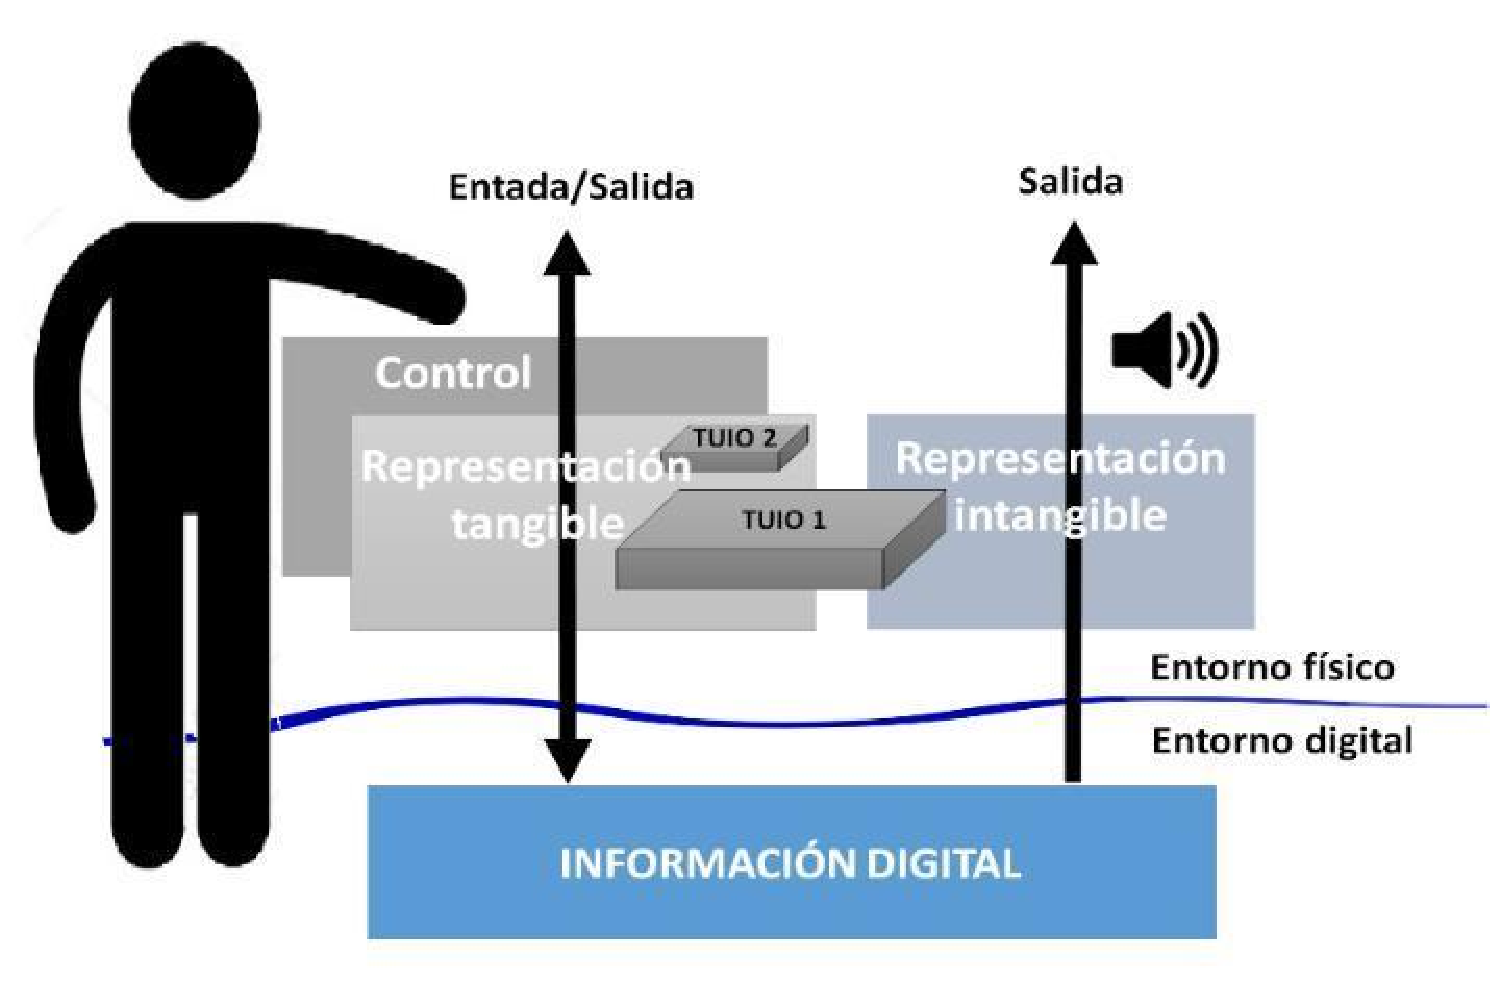
\includegraphics[width=0.5\textwidth]{SIS.pdf}
\caption{Modelo de interacción de interfaz TUI para este proyecto}
\label{fig:SIS}
\end{center}
\end{figure}

El sistema de juego propuesto abarca desde el desarrollo de una secuencia, a partir de los criterios de creación del niño, hasta la resolución de pequeños problemas de lógica. El elemento TUIO1 consta de una pantalla táctil, encargada de la representación gráfica tangible e intangible del juego. Si bien los elementos tangibles juegan el papel central en la representación y control en un TUI, la representación intangible es también importante, añadiendo gráficos y audio, siendo esta información dinámica proporcionada, una gran ayuda a la hora de la realización de la interacción. 

La existencia en tiempo real de una realimentación de la representación intangible, cuando se ha manipulado la representación tangible, es fundamental para asegurar un correcto acoplamiento perceptivo. Las representaciones intangibles que incorpora el diseño, son tanto auditivas, producidas en determinados puntos del desarrollo del juego, como gráficas, mostrando en determinadas zonas de la pantalla táctil, información no modificable por el usuario.
Los componentes, y los eventos que se producen en la interacción, junto con las comunicaciones con TUIO2, están controladas mediante un microprocesador.

El segundo elemento tangible TUIO2, actúa como elemento de programación tangible, agrupando funciones,
características y elementos que pueden ser aplicados al juego, y que facilitan las interacciones o
modificaciones a efectuar sobre el juego. Uno de los factores principales de las interfaces tangibles, es el acoplamiento de las representaciones tangibles a información digital y modelos computacionales. 

Uno de los retos en el diseño de TUI, es como mapear los objetos físicos y como realizar una manipulación a la computación digital y la retroalimentación de una manera significativa y completa.
Para solucionar el problema de disponer de distintos elementos tangibles para el desarrollo del juego, el dispositivo TUIO2 hace de puente entre la interfaz física y la digital, agrupando todos los elementos de interacción en un solo dispositivo. 

Al disponer de una pantalla táctil se hace más intuitivo y sencillo el uso de este elemento tangible. Además de una pantalla táctil dispone de sensores de posicionamiento y orientación. Estos componentes y los eventos producidos son tratados en un microcontrolador, el cual también es el encargado de las comunicaciones con el dispositivo TUIO1.



\section{Objetivo general}

Diseñar y desarrollar una plataforma interactiva de juego de bajo coste, basada en interfaces tangibles, para promover el desarrollo de capacidades en niños de corta edad.

\section{Objetivos específicos}

\begin{itemize}
\item Diseñar y programar un sistema de localizacion y reconocimiento de las interfaces de usuario tangibles.

\item Desarrollar un sistema eficiente de transferencia de datos entre ambas interfaces tangibles.

\item Realizar una correcta sincronización en la visualización de la aplicación entre ambas pantallas, que permita una buena representación de juego.

\item Ofrecer un entorno gráfico simple, que permita al niño ser capaz de diseñar secuencias y modificarlas interactuando con los elementos tangibles.

\item Adaptar sensores inerciales y ópticos para una mejor experiencia de juego, donde ambos elementos tangibles interactúen entre sí, permitiendo la manipulación de la información entre los dispositivos.

\item Diseñar un sistema de actualización de software de los dispositivos, a través de la conexión externa a un servidor.
\end{itemize}



% Local Variables:
%  coding: utf-8
%  mode: latex
%  mode: flyspell
%  ispell-local-dictionary: "castellano8"
% End:
